\documentclass{article}
\usepackage[utf8]{inputenc}
\usepackage{physics}
\usepackage{amsmath}
\usepackage{showlabels}
\usepackage{amssymb}
\title{Statistical Computing for Scientists and Engineers\\[1em] Homework 3}
\author{Jiale Shi}
\date{September/21/2018}

\usepackage{natbib}
\usepackage{graphicx}
\usepackage{array}
\begin{document}
\maketitle

\newpage
\section{Problem 1}
The problem of interest consists of a scalar output $y$ (the logarithmic of the number of caterpillars colonies in a $500 m^2$ area) and $k=10$ explanatory variables $x_{i} (i=1,...,10)$ which correlate to features such as altitude, landscape slope, vegetation count, etc. The exact meaning does not matter in this context. Using the caterpillar.mat data, plot the semi-log-y plots of the caterpillar colony (last column of the data file) versus each feature reproducing Figure 3.1 in Bayesian Core.

Answer: we run the code that provided to us. We get the semi-log-$y$ plots are shown below.

\begin{figure}[h!]
\centering
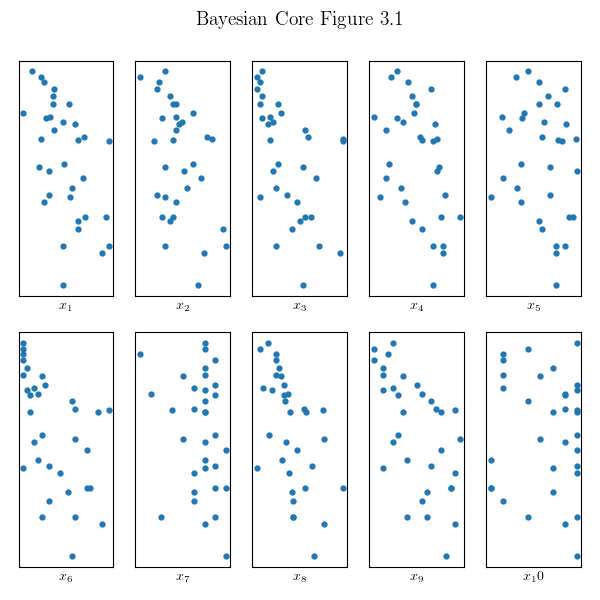
\includegraphics[scale=0.6]{Figure3_1.png}
\caption{semi-$\log$-$y$ plots}
%\label{fig:universe}
\end{figure}




\newpage
\section{Problem 2}
From the book, 3.1.1 linear model

The ordinary normal linear regression model is such that 
\begin{equation}
    y|\beta,\sigma^{2},X \sim \mathcal{N}_{n}(X\beta,\sigma^{2}I_{n})
\end{equation}

the likelihood of the ordinary normal linear model is
\begin{equation}
    l(\beta,\sigma^{2}|y,X) = (2\pi\sigma^{2})^{n/2} \exp\left[-\frac{1}{2\sigma^2}(y-X\beta)^{T}(y-X\beta)\right]
\end{equation}

The maximum likelihood estimator of $\beta$ is then the solution of the (least squares) minimization problem.

\begin{equation}
\min_{\beta}(y-X\beta)^{T}(y-X\beta) = \min_{\beta}\sum_{i=1}^{n}(y_{i}-\beta_{0}-\beta_{1}x_{i1}-...-\beta{k}x_{ik})^2    
\end{equation}
namely,
\begin{equation}
\hat{\beta} = (X^{T} X)^{-1}X^{T}y    
\end{equation}
which is also the orthogonal projection of y on the linear subspace spanned by the columns of $X$.

Similarly, an unbiased estimator of $\sigma^{2}$ is
\begin{equation}
  \hat{\sigma}^2 = \frac{1}{n-k-1}(y-X\hat{\beta})^{T} (y-X\hat{\beta}) = \frac{s^{2}}{n-k-1}
\end{equation}
and $\hat{\sigma}^2(X^{T}X)^{-1}$ approximates the covariance matrix of $\hat{\beta}$. We can then define the standard t-statistic as 

\begin{equation}
    T_{i} = \frac{\hat{\beta}_{i}-\beta_{i}}{\sqrt{\hat{\sigma}^2\omega_{(i,i)}}} ~\mathcal{J}_{n-k-1} = 
\end{equation}
where $\omega_{(i,i)}$ denotes the $(i,i)$th element of the matrix $(X^{T}X)^{-1}$. For this problem $\beta_{i}=0$ 

the p value
\begin{equation}
    p_{i}= P_{H_{0}}(|T_{i}|-|t_{i}|) < \alpha
\end{equation}

Note that this statistic $T_{i}$ can also be used to build on the $\beta_{i}$s as a (marginal) frequentist confidence interval, of the form.

\begin{equation}
    {\beta_{i};|\beta_{i}-\hat{\beta}_{i}|<=\sqrt{\omega_{ii}}F^{-1}_{n-k-1}(1-\alpha/2)}
\end{equation}

Then we run the code that is offered to us. We reproduce Figure 3.2
\begin{figure}[h!]
\centering
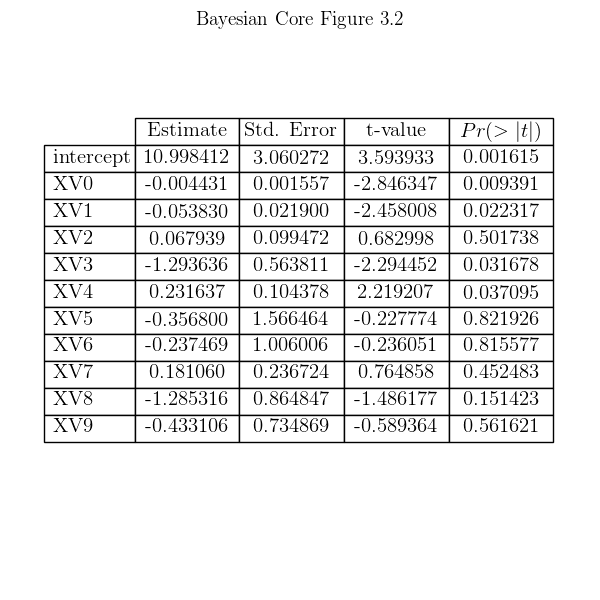
\includegraphics[scale=0.6]{Figure3_2.png}
\caption{Dataset caterpillar: output providing the maximum likelihood estimates of the regression coefficients and their standard significance analysis.}
%\label{fig:universe}
\end{figure}


\section{Problem 3}
We mainly focus on the section 3.2.1 Conjugate Priors.

We use the conjugate prior:
\begin{equation}
\begin{aligned}
    &\beta|\sigma^{2}, X \sim \mathcal{N}_{k+1}(\Tilde{\beta},\sigma^{2}M^{-1})  \\
    &\sigma^{2} | X \sim \mathcal{IG}(a,b)
\end{aligned}
\end{equation}
%Use the hyper-parameter values of $\Tilde{\beta}$,k=10,a=2.1andb=2.0forcomputingthetablevalues.
The prior is conjugate, leading us to the following normal-inverse-gamma posterior distribution.

\begin{equation}
\begin{aligned}
    &\beta|\sigma^{2},y, X \sim \mathcal{N}_{k+1}((M+X^{T}X)^{-1}X^{T}X\Tilde{\beta},\sigma^{2}[M^{-1}+(X^{T}X)^{-1}]^{-1})  \\
    &\sigma^{2} | y,X \sim \mathcal{IG}(\frac{n}{2},b+\frac{s^2}{2}+\frac{\hat{\beta}^{T}[M^{-1}+(X^{T}X)^{-1}]^{-1}\hat{\beta}}{2})
\end{aligned}
\end{equation}
In this setting, the Bayes estimators of $\beta$ and $\sigma^{2}$ associated with squared error losses, namely the posterior means of $\beta$ and $\sigma^{2}$, can be computed in closed form. In fact, a simple computation shows that they are given by
\begin{equation}
\begin{aligned}
    \mathbb{E}^{\pi}[\beta|y,X] &= \mathbb{E}^{\pi}[\mathbb{E}^{\pi}(\beta|\sigma^2,y,X)|y,X] \\
    & = (M+X^{T}X)^{-1}{(X^{T}X)\hat{\beta}+M\hat{\beta}}
\end{aligned}
\end{equation}

and for $n\geq 2$

\begin{equation}
\begin{aligned}
    \mathbb{E}^{\pi}[\beta|y,X] &= \frac{2b+s^{2}+(\tilde{\beta}-\hat{\beta})^{T}{M^{-1}+(X^{T}X)^{-1}}^{-1}(\tilde{\beta}-\hat{\beta})}{n+2a-2}
\end{aligned}
\end{equation}

Integrating Eq.10 in $\sigma^{2}$ leads to a multivariate $t$ marginal posterior distribution on $\beta$ since.

\begin{equation}
\begin{aligned}
\pi(\beta|y,X) & \propto [ (\beta-{M+X^{T}X}^{-1}[{X^{T}X}\hat{\beta}+M\tilde{\beta}])^{T} (M+X^{T}X)  \\
&\times (\beta-{M+X^{T}X}^{-1}[{X^{T}X}\hat{\beta}+M\tilde{\beta}]) +2b+s^2  \\
&+(\tilde{\beta}-\hat{\beta})^{T} (M^{-1}+(X^{T}X)^{-1})^{-1} (\tilde{\beta}-\hat{\beta})
]^{-(n/2+k/2+a)}
\end{aligned}
\end{equation}

We thus have that, marginally and a posteriori,
\begin{equation}
    \beta|y,X \sim \mathcal{J}_{k+1}(n+2a,\hat{\mu},\hat{\Sigma})
\end{equation}

with 
\begin{equation}
\begin{aligned}
    & \hat{\mu} = (M+X^{T}X)^{-1}((X^{T}X)\hat{\beta}+M\tilde{\beta}) \\
    & \hat{\Sigma} = \frac{2b+s^2 +(\tilde{\beta}-\hat{\beta})^{T} (M^{-1}+(X^{T}X)^{-1})^{-1} (\tilde{\beta}-\hat{\beta})}{n+2a}(M+X^{T}X)^{-1}
\end{aligned}
\end{equation}

\begin{equation}
\begin{aligned}
    \mathbb{V}^{\pi} &= \frac{n+2a}{n+2a-4} \hat{\Sigma} \\
    &=  \frac{2b+s^2 +(\tilde{\beta}-\hat{\beta})^{T} (M^{-1}+(X^{T}X)^{-1})^{-1} (\tilde{\beta}-\hat{\beta})}{n+2a-4}(M+X^{T}X)^{-1}
\end{aligned}
\end{equation}

\begin{figure}[h!]
\centering
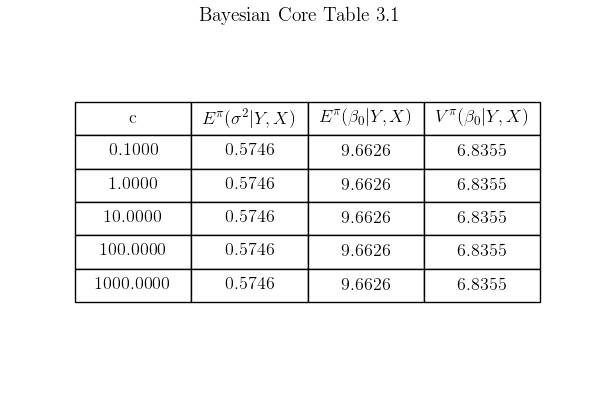
\includegraphics[scale=0.6]{Table3_1.png}
\caption{Dataset caterpillar: Influence of the prior scale c on the Bayes estimates of $\sigma^2$ and $\beta_{0}$.}
%\label{fig:universe}
\end{figure}

\begin{figure}[h!]
\centering
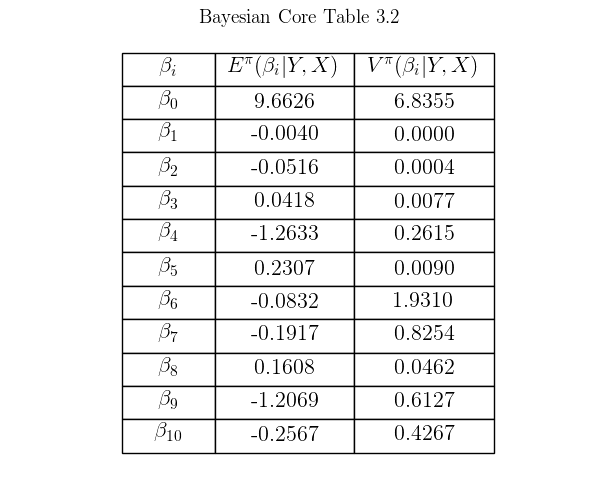
\includegraphics[scale=0.6]{Table3_2.png}
\caption{Dataset caterpillar: Bayes estimates of $\beta$ for $c=100$.}
%\label{fig:universe}
\end{figure}

\newpage
\section{Problem 4}
The posterior distribution can be  derived as 
\begin{equation}
\begin{aligned}
    \pi(\beta,\sigma^2|y,X) & \propto f(y|\beta,\sigma^2,X)\pi(\beta,\sigma^2|X) \\
    &\propto (\sigma^{2})^{-n/2-1} \exp [-\frac{1}{2\sigma^2}(y-X\hat{\beta})^{T}(y-X\hat{\beta})-\frac{1}{2\sigma^2}(\beta-\hat{\beta})^{T}(X^{T}X)(\beta-\hat{\beta})]\\
    &\cdot (\sigma^2)^{-k/2} \exp[-\frac{1}{2c\sigma^2}(\beta^T X^T X\beta)]
\end{aligned}
\end{equation}
Conduct marginalization and derive the conditional and marginal posteriors on $\beta$ and $\sigma^{2}$:

\begin{equation}
\begin{aligned}
    & \beta | \sigma^{2},y, X \sim \mathcal{N}_{k+1}(\frac{c}{c+1}\hat{\beta}, \frac{\sigma^2 c}{c+1}(X^{T} X)^{-1}) \\
     & \sigma^2 | y, X \sim \mathcal{IG}(\frac{n}{2}, \frac{s^2}{2}+\frac{1}{2(c+1)}\hat{\beta}^T X^T X \hat{\beta}) \\
\end{aligned}
\end{equation}


By integrating out $\sigma^2$ on the conditional posterior $\beta$, we can show that
\begin{equation}
\begin{aligned}
    \beta | y,X \sim \mathbb{T}_{k+1} (n,\frac{c}{c+1}\hat{\beta},\frac{c(s^2+\frac{\hat{\beta}^{T} X^{T} X \hat{\beta}}{c+1})}{n(c+1)}(X^T X)^{-1})
\end{aligned}
\end{equation}

\begin{equation}
\begin{aligned}
    & \mathcal{E}[\beta|y,X] = \frac{c}{c+1} \hat{\beta} \\
    & \mathcal{V}[\beta|y,X] = \frac{c(s^2+\frac{\hat{\beta}^{T} X^{T} X \hat{\beta}}{c+1})}{(n-2)(c+1)}(X^T X)^{-1}
\end{aligned}
\end{equation}

And the expression of Bayes factor has been given.

\begin{figure}[h!]
\centering
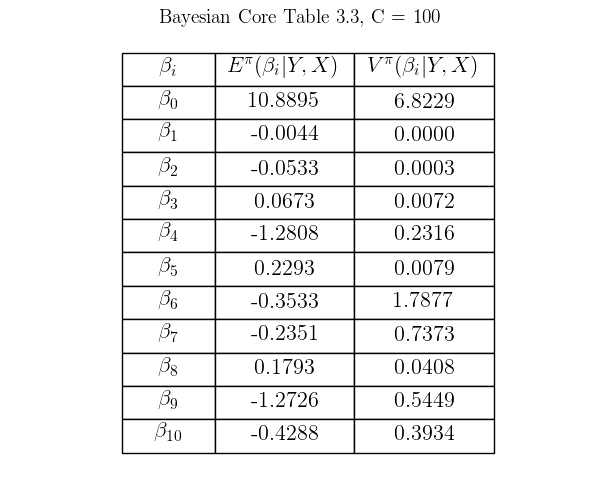
\includegraphics[scale=0.6]{Table3_3.png}
\caption{Dataset caterpillar: Posterior mean and variance of $\beta$ for $c=100$ using Zellar's G-prior.}
%\label{fig:universe}
\end{figure}

\begin{figure}[h!]
\centering
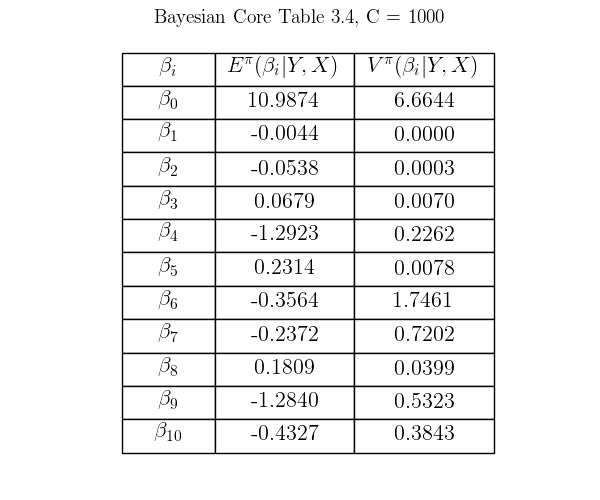
\includegraphics[scale=0.6]{Table3_4.png}
\caption{Dataset caterpillar: Same legend as Table 3.3 for c=1000}
%\label{fig:universe}
\end{figure}

The dependence of the Bayes factor on the pair ($c,c_{0}$) cannot be bypassed in the sense that the Bayes factor varies between $0$ and $\infty$ when $c_{0}/c$ goes from $0$ to $\infty$. 

Although these Bayes factors should not be used simultaneously, an informal conclusion is that the most important variables besides the intercept seem to be $X_{1},X_{2},X_{4}$ and $X_{5}$.

\newpage
\section{Problem 5}
The marginal posterior distribution from Problem 4:

\begin{equation}
\begin{aligned}
    \beta | y,X \sim \mathbb{T}_{k+1} (n,\frac{c}{c+1}\hat{\beta},\frac{c(s^2+\frac{\hat{\beta}^{T} X^{T} X \hat{\beta}}{c+1})}{n(c+1)}(X^T X)^{-1})
\end{aligned}
\end{equation}

As the standard student-t is one symmetrical distribution, we can analytically calculate its $90\%$ HPD region as the two points whose respective CDF is $5\%$ and $95\%$. Denote them as $\delta_{5}$ and $\delta_{95}$. The corresponding HPD of $\beta$ would than be

\begin{equation}
\begin{aligned}
    & \beta_{5} = \frac{c}{c+1}\hat{\beta} + \delta_{5} \cdot \frac{c(s^2+\frac{\hat{\beta}^{T} X^{T} X \hat{\beta}}{c+1})}{n(c+1)}(X^T X)^{-1}) \\
    & \beta_{95} = \frac{c}{c+1}\hat{\beta} + \delta_{95} \cdot \frac{c(s^2+\frac{\hat{\beta}^{T} X^{T} X \hat{\beta}}{c+1})}{n(c+1)}(X^T X)^{-1}) 
\end{aligned}
\end{equation}

\begin{figure}[h!]
\centering
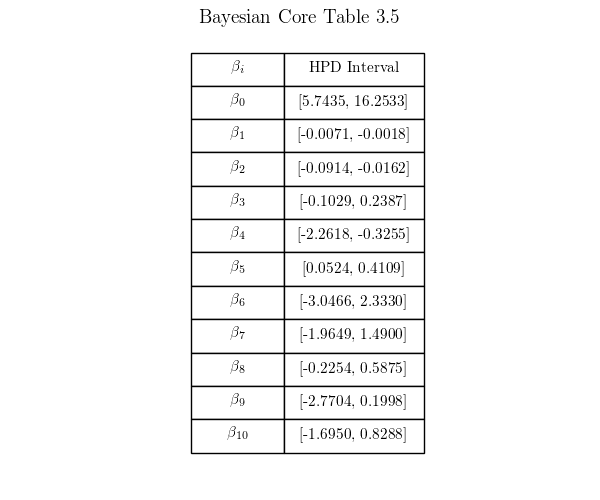
\includegraphics[scale=0.6]{Table3_5.png}
\caption{Dataset caterpillar:$95\%$ HPD intervals for the components of $\beta$ for $c=100$}
%\label{fig:universe}
\end{figure}

\newpage
\section{Problem 6}
We now consider c an unknown hyper-parameter, that is we use the same G-prior distribution, and we now introduce a diffuse prior distribution on c.

\begin{equation}
\begin{aligned}
    \pi(c)=c^{-1} \mathcal{I}_{\mathcal{N*}}(c)
\end{aligned}
\end{equation}

the corresponding marginal posterior on the parameters of interest is then
\begin{equation}
\begin{aligned}
    \pi(\beta,\sigma^2|y,X) \sum_{c=1}^{\infty} \pi(\beta,\sigma^{2}|y,X,c)f(y|X,c)c^{-1}
\end{aligned}
\end{equation}

\begin{equation}
\begin{aligned}
    f(y|X) &\propto_{c} f(y|X,c)\pi(c) \\
    & \sum_{c}c^{-1}(c+1)^{-\frac{k+1}{2}} [y^T y-\frac{c}{c+1}y^T X(X^T X)^{-1} X^{T} y]^{-n/2}
\end{aligned}
\end{equation}

For the posterior mean and variance of $\beta$, we integrate out $c$ by summation:
\begin{equation}
\begin{aligned}
    \mathcal{E}[\beta|y,X] = \sum_{c}\mathcal{E}[\beta|y,X,c]\pi(c|y,X)
\end{aligned}
\end{equation}

because $\pi(c|y,X) \propto f(y|X,c) \pi(c)$

\begin{equation}
\begin{aligned}
    \mathcal{E}[\beta|y,X] = \sum_{c} \frac{c}{c+1} \hat{\beta} \pi(c|y,X) = \hat{\beta} \sum_{c} [\frac{c}{c+1}\frac{f(y|X,c)\pi(c)}{\sum_{c}f(y|X,c)\pi(c)}]
\end{aligned}
\end{equation}

\begin{equation}
\begin{aligned}
    \mathcal{V}[\beta|y,X] = \mathcal{E}[\mathcal{V}(\beta|y,X,c)|y,X] + \mathcal{V}(\mathcal{E}[\beta,X,c]|y,X)
\end{aligned}
\end{equation}

\begin{figure}[h!]
\centering
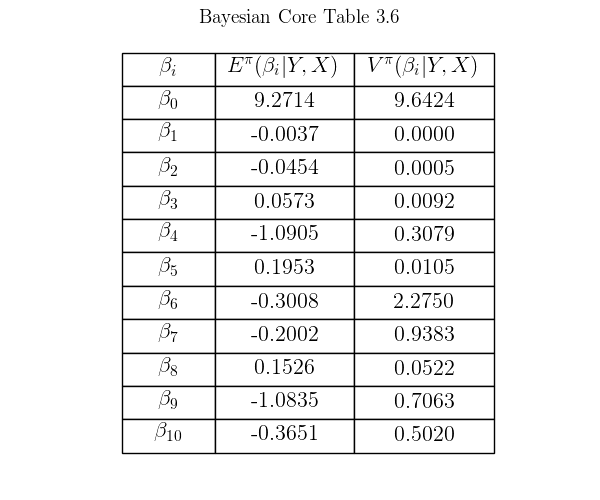
\includegraphics[scale=0.6]{Table3_6.png}
\caption{Table of Problem 6}
%\label{fig:universe}
\end{figure}

An important point with this approach is that the marginal distribution of the dataset is available in closed form. It is therefore possible to produce a Bayes regression output, just as in the first-level prior. This is one additional reason why this non-informative prior is introduced.

\newpage
\section{Problem 7}

The algorithm is stochastic search for the most likely model.
When k is large, it becomes computationally intractable to compute the posterior probabilites of the $2^{k}$ models. Need of a tailored algorithm that samples from $p(\gamma|y, X)$ and selects the most likely models.
This can be done by Gibbs sampling, given the availability of the full conditional posterior probabilities of the $\gamma_{i}$'s.
If the $\pi$ with the that model parameter is much larger than that without that model parameter, that model parameter should be turned on. 
If the $\pi$ with the that model parameter is much smaller than that without that model parameter, that model parameter should be turned off. 

\begin{figure}[ht]
\centering
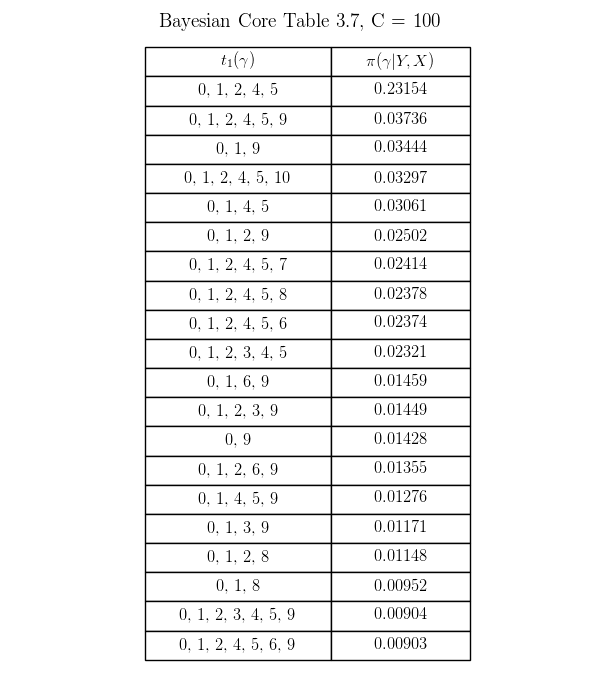
\includegraphics[scale=0.6]{Table3_7.png}
\caption{Table of Problem 7(a)}
%\label{fig:universe}
\end{figure}

\begin{figure}[ht]
\centering
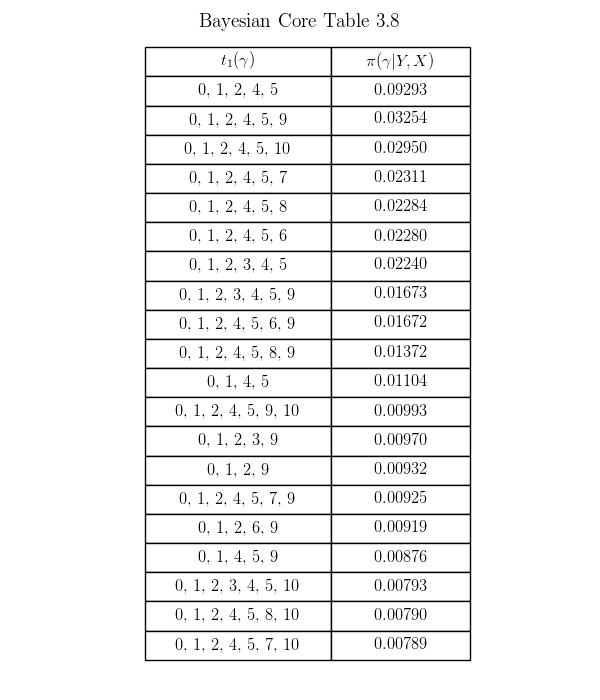
\includegraphics[scale=0.6]{Table3_8.png}
\caption{Table of Problem 7(b)}
%\label{fig:universe}
\end{figure}

\begin{figure}[ht]
\centering
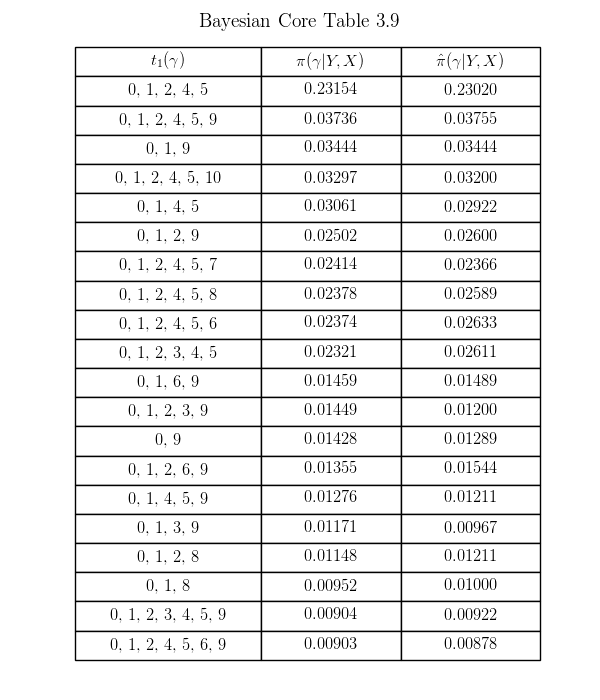
\includegraphics[scale=0.6]{Table3_9.png}
\caption{Table of Problem 7(c)}
%\label{fig:universe}
\end{figure}


\begin{figure}[ht]
\centering
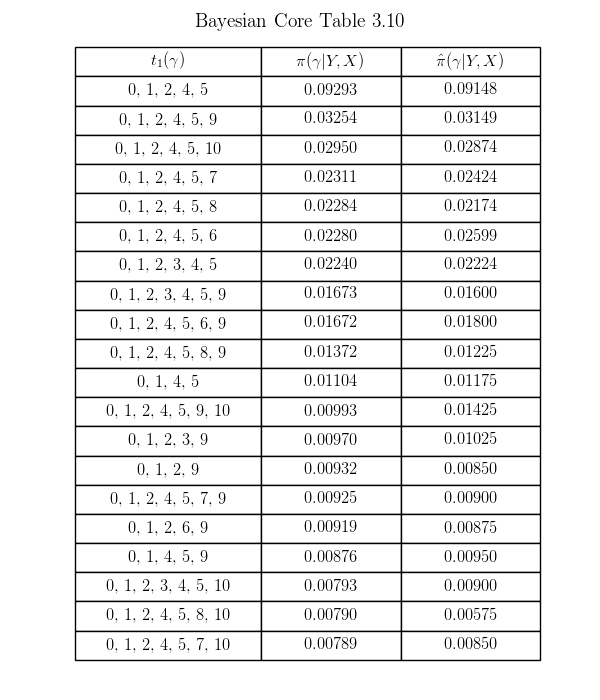
\includegraphics[scale=0.6]{Table3_10.png}
\caption{Table of Problem 7(d)}
%\label{fig:universe}
\end{figure}

\begin{figure}[ht]
\centering
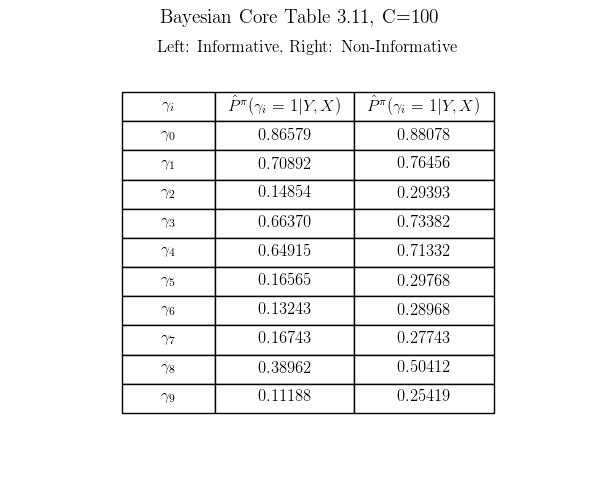
\includegraphics[scale=0.6]{Table3_11.png}
\caption{Table of Problem 7(e)}
%\label{fig:universe}
\end{figure}


%\bibliographystyle{plain}
%\bibliography{references}
\end{document}
